

\section{Schwachstelle 13: Unsicheres WLAN-Passwort der SSID \texttt{Mickey's Office}}
\label{sec:vuln13}
Der aus Schwachstelle 12 erhaltene Netzwerkmittschnitt des \texttt{Lightman}-Benutzers enthält einen WLAN-Trace des \texttt{Mickey's Office}-WLAN, welches mit einem schwachen WPA2-PSK Passwort abgesichert ist.

\subsection{Beschreibung der Schwachstelle}
\label{subsec:vuln13_way}


Eine erste Analyse des Netzwerksmitschnitts der Datei \texttt{MickeyOfficeDump-01.cap} mit Wireshark hatte ergeben, dass das WLAN \texttt{Mickey's Office} (BSSID des Access-Points: \texttt{90:F6:52:3E:2E:38}) und der WLAN-Client mit der MAC-Adresse \texttt{00:21:5C:75:B4:27} mit einer Deauthentication-Attacke angegriffen wurden, um anschließend einen 4-Wege-Handhsake des WPA-Protokolls abzufangen.

Über das Wireshark-Menü \texttt{Wireless -> WLAN Traffic} kann die in Abbildung \ref{wlan_trace_stats} gezeigte Statistik eingesehen werden. Diese verdeutlicht anhand der Spalte \texttt{Deauths}, dass eine Deauthentication-Attacke mit 3630 Paketen durchgeführt wurde.

\begin{figure}[h]
    \centering
    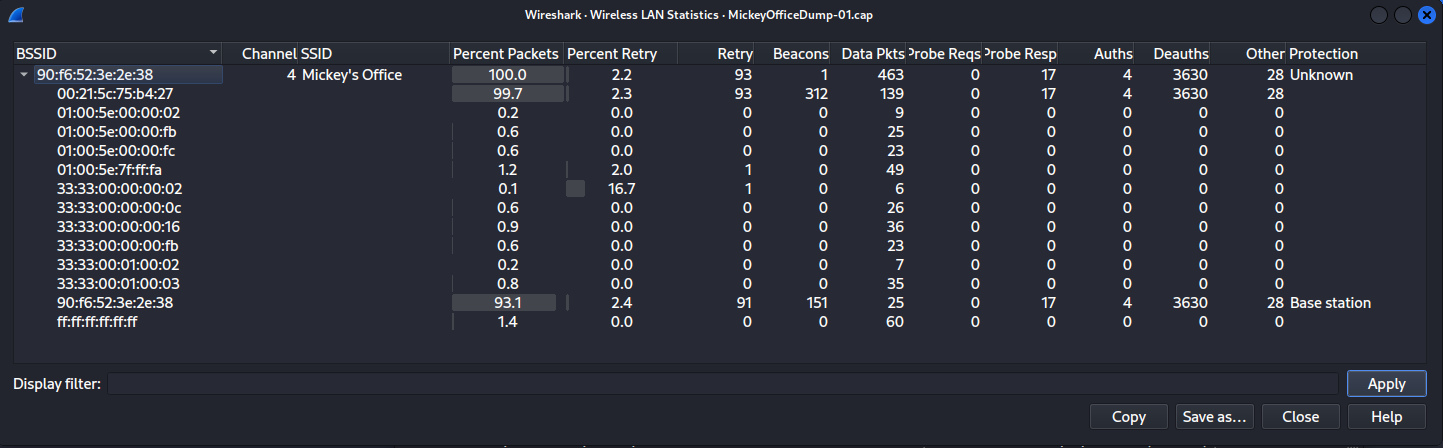
\includegraphics[width=\textwidth]{./img/vuln11_inside/wlan_trace_stats}
    \caption{Wireshark-Statistikdaten des \texttt{MickeyOfficeDump-01.cap}-Traces.}
    \label{wlan_trace_stats}
\end{figure}

Die Ausgabe des Befehls \texttt{airodump-ng -r MickeyOfficeDump-01.cap} zeigt weiterhin, dass es sich bei dem WLAN \texttt{Mickey's Office} um ein WPA2 (CCMP) geschütztes WLAN mit einem Pre-Shared-Key (PSK) handelt  (s. Textauszug \ref{lst:vuln13_airodump}).

\lstset{language=bash,caption={Ausgabe des Befehls \texttt{airodump-ng -r MickeyOfficeDump-01.cap}.}, label=lst:vuln13_airodump}
\begin{lstlisting}[frame=single, firstnumber=1, stepnumber=1,]
|--(gu4c4m0l3@kali-t470)-[~/Documents/pentest_MB-Reps/esperanza]
|-$ airodump-ng -r MickeyOfficeDump-01.cap

 CH  0 ][ Elapsed: 24 s ][ 2022-03-03 22:20 ][ Are you sure you want to quit? Press Q again to quit.                                                                                                                                                                                                                        
                                                                                                                                                                                                                                                                                                                            
 BSSID              PWR  Beacons    #Data, #/s  CH   MB   ENC CIPHER  AUTH ESSID                                                                                                                                                                                                                                            
                                                                                                                                                                                                                                                                                                                            
 90:F6:52:3E:2E:38    0        1      467    0   4  270   WPA2 CCMP   PSK  Mickey's Office                                                                                                                                                                                                                                  
                                                                                                                                                                                                                                                                                                                            
 BSSID              STATION            PWR   Rate    Lost    Frames  Notes  Probes                                                                                                                                                                                                                                          
                                                                                                                                                                                                                                                                                                                            
 90:F6:52:3E:2E:38  00:21:5C:75:B4:27    0    0e- 0e     0     2173  EAPOL                                                                                                                                                                                                                                                  
\end{lstlisting} 

Des Weiteren zeigt Abbildung \ref{wlan_trace_handshake}, den Wireshark-Filter \texttt{eapol} mit den dazugehörigen Handshake-Nachrichten. Diese ermöglichen einem Angreifer mit dem Befehl \texttt{hcxpcapngtool -o pmkid-handshakes.hccapx MickeyOfficeDump-01.cap}\footnote{Um den Befehl ausführen zu können müssen die \texttt{hcxtools}-Pakete mit dem Befehl \texttt{sudo apt install hcxdumptool hcxtools } auf der Kali-VM nachinstalliert werden.} den Hashwert des WPA2-Passworts in die Datei \texttt{pmkid-handshakes.hccapx} zu extrahieren (s. Abbildung \ref{hcxpcapngtool}). Textausgabe \ref{lst:vuln13_wpa2hash} stellt den Inhalt der Datei \texttt{pmkid-handshakes.hccapx} mit dem WPA2-Hashwert dar.

\begin{figure}[h]
    \centering
    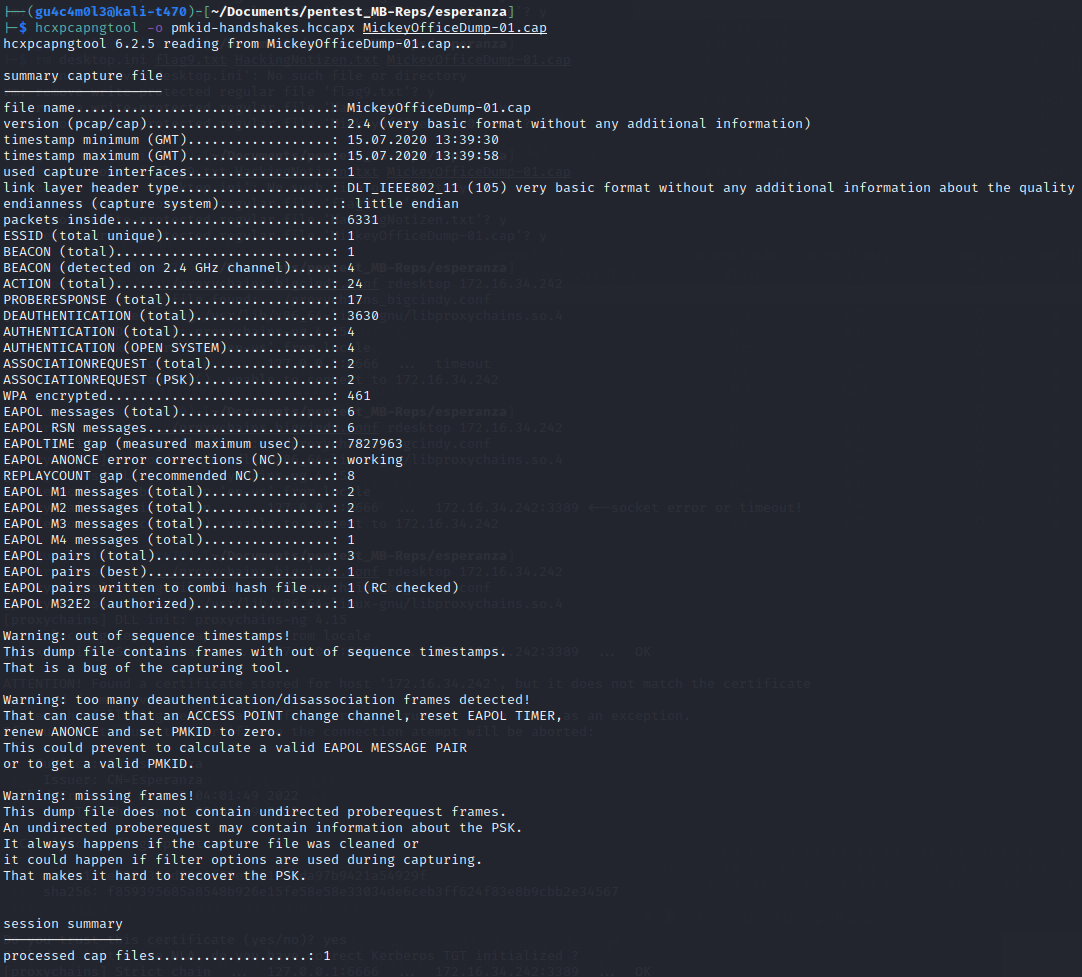
\includegraphics[width=\textwidth]{./img/vuln13_mickey/hcxpcapngtool}
    \caption{Extrahieren des WPA2-Hashwertes mit \texttt{hcxpcapngtool}.}
    \label{hcxpcapngtool}
\end{figure}


\begin{figure}[h]
    \centering
    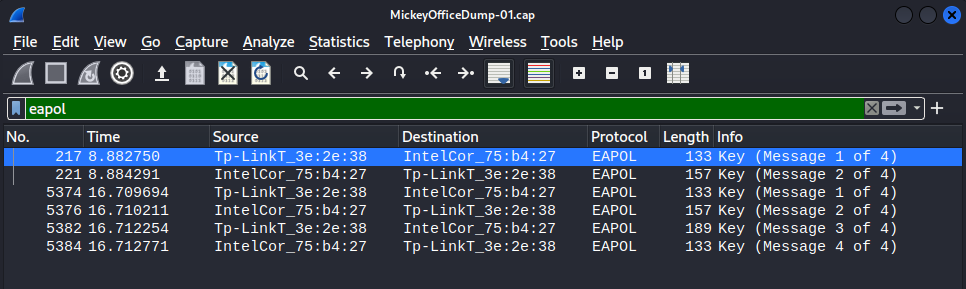
\includegraphics[width=\textwidth]{./img/vuln11_inside/wlan_trace_handshake}
    \caption{Erzwungener WPA-Handshake aufgrund Deauth-Attacke.}
    \label{wlan_trace_handshake}
\end{figure}

\lstset{language=bash,caption={WPA2-Hashwert des WLANs \texttt{Mickey's Office}.}, label=lst:vuln13_wpa2hash}
\begin{lstlisting}[frame=single, firstnumber=1, stepnumber=1,]
|--(gu4c4m0l3@kali-t470)-[~/Documents/pentest_MB-Reps/esperanza]
|-$ cat pmkid-handshakes.hccapx               
WPA*02*296244d3ab119eb009a491aac042cfe1*90f6523e2e38*00215c75b427*4d69636b65792773204f6666696365*2592cabe58c6b152c2e78f8818b551f3cb4a723abee73a9870ecaeee17f3a65d*0103007702010a00000000000000000001eb8b5453b691834c93e94b98d05990edad250e6934247f085b62f e2b26329920000000000000000000000000000000000000000000000000000 000000000000000000000000000000000000000000000001830160100000fac040100000fac040100000fac023c000000*a2
\end{lstlisting} 


Anschließend kann das WLAN-Passwort mit dem Hashcat-Befehl \texttt{hashcat -m 22000 -a 0 pmkid-handshakes.hccapx /usr/share/wordlists/rockyou.txt} wie in Abbildung \ref{mickey_hashcat} dargestellt gebrochen werden. Das Passwort zum WLAN \texttt{Mickey's Office} lautet \texttt{basketball4va\#12}.

\begin{figure}[h]
    \centering
    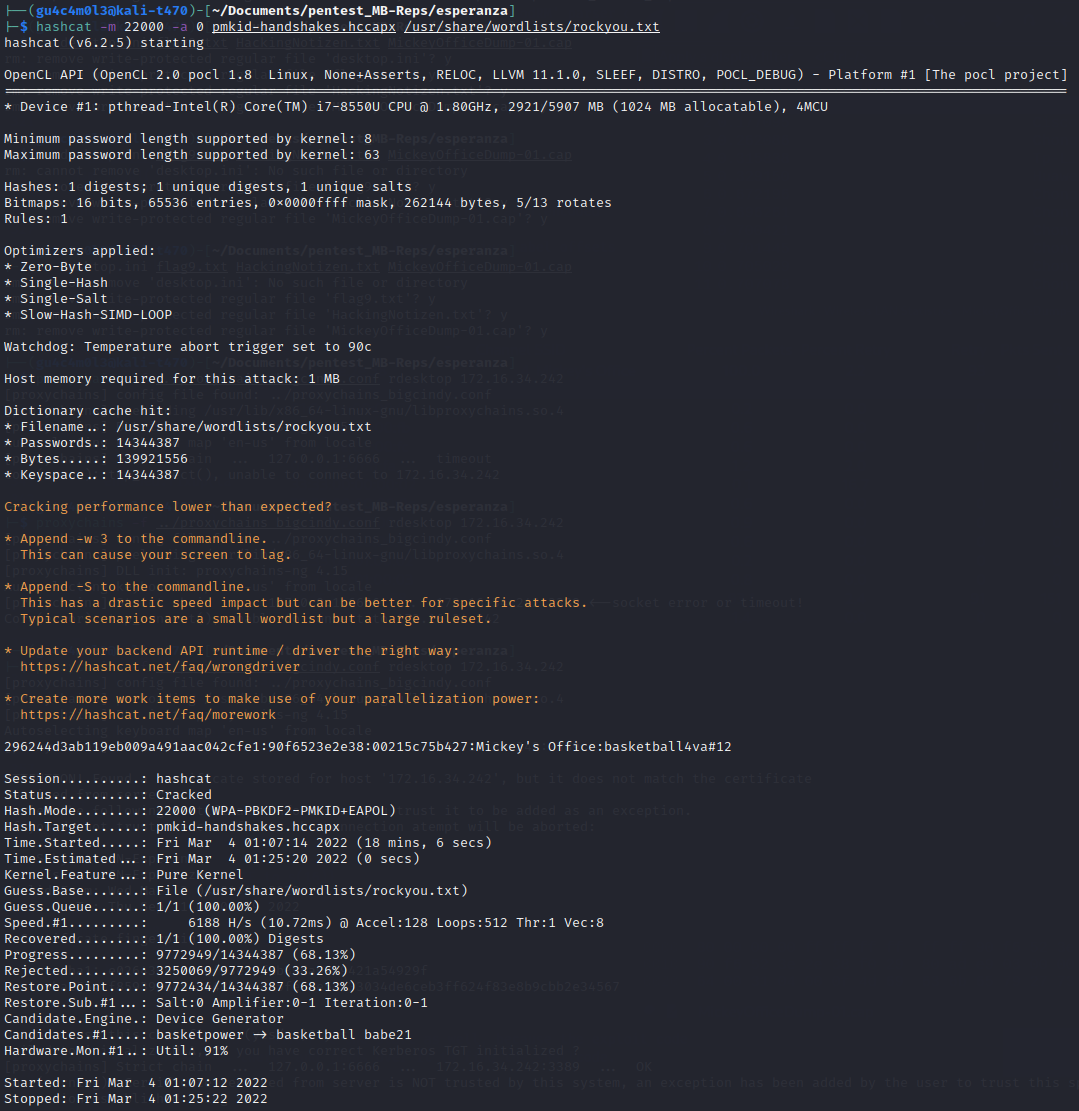
\includegraphics[width=\textwidth]{./img/vuln13_mickey/hashcat}
    \caption{Hashcat-Befehl zum brechen des WLAN-Passworts.}
    \label{mickey_hashcat}
\end{figure}

Abbildung \ref{mickey_login} zeigt abschließend, wie der Benutzer \texttt{mickey} auf den Host \texttt{Mickey} (IP: \texttt{172.16.34.224}) mit dem soeben gebrochenem WLAN-Passwort \texttt{basketball4va\#12} über SSH anmeldet. Der Benutzer \texttt{mickey} ist darüber hinaus Mitglied der \texttt{sudo}-Gruppe und kann somit beliebige Befehl unter Root-Berechtigungen ausführen (s. Abbildung \ref{mickey_root}).






\begin{figure}[h]
    \centering
    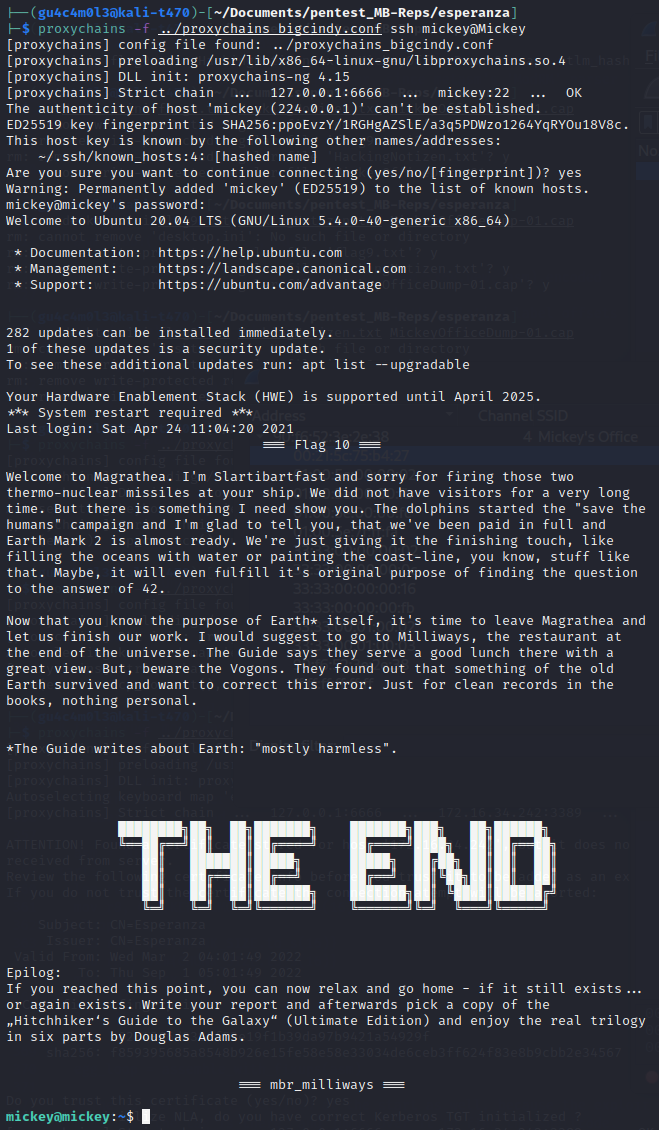
\includegraphics[width=0.85\textwidth]{./img/vuln13_mickey/mickey_login}
    \caption{SSH-Login auf den Host \texttt{Mickey} mit dem aus dem WLAN gebrochenem Passwort.}
    \label{mickey_login}
\end{figure}

\begin{figure}[h]
    \centering
    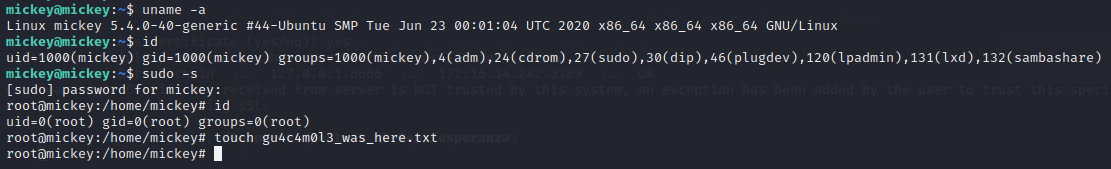
\includegraphics[width=\textwidth]{./img/vuln13_mickey/mickey_root}
    \caption{\texttt{sudo}-Gruppenmitgliedschaft von \texttt{mickey} erlaubt Root-Berechtigungen.}
    \label{mickey_root}
\end{figure}


Textauszug \ref{lst:mickey_graphical} verdeutlicht, dass neben reinen SSH-Sitzungen mit dem Paramter \texttt{-X} der SSH-Sitzung auch grafische Applikationen über X11 gestartet werden können. So zeigt Abbildung \ref{gnome-control-center} die Ausführung der grafischen Applikation \texttt{gnome-control-center} und stellt die Systeminformationen der Ubuntu 20.04 LTS Maschine dar.


\lstset{language=bash,caption={Starten von grafischen Applikationen über den \texttt{-X}-Parameter der SSH-Sitzung.}, label=lst:mickey_graphical}
\begin{lstlisting}[frame=single, firstnumber=1, stepnumber=1,]
|--(gu4c4m0l3@kali-t470)-[~/Documents/pentest_MB-Reps/esperanza]
|-$ proxychains -f ../proxychains_bigcindy.conf ssh -X mickey@Mickey                                                                                                                                                                          
[proxychains] config file found: ../proxychains_bigcindy.conf
[proxychains] preloading /usr/lib/x86_64-linux-gnu/libproxychains.so.4
[proxychains] DLL init: proxychains-ng 4.15
[proxychains] Strict chain  ...  127.0.0.1:6666  ...  mickey:22  ...  OK
mickey@mickey's password: 
[proxychains] DLL init: proxychains-ng 4.15
                                           Welcome to Ubuntu 20.04 LTS (GNU/Linux 5.4.0-40-generic x86_64)
        
        [... Ausgabe gekürzt ...]

mickey@mickey:~$ gnome-control-center 
\end{lstlisting} 

\begin{figure}[h]
    \centering
    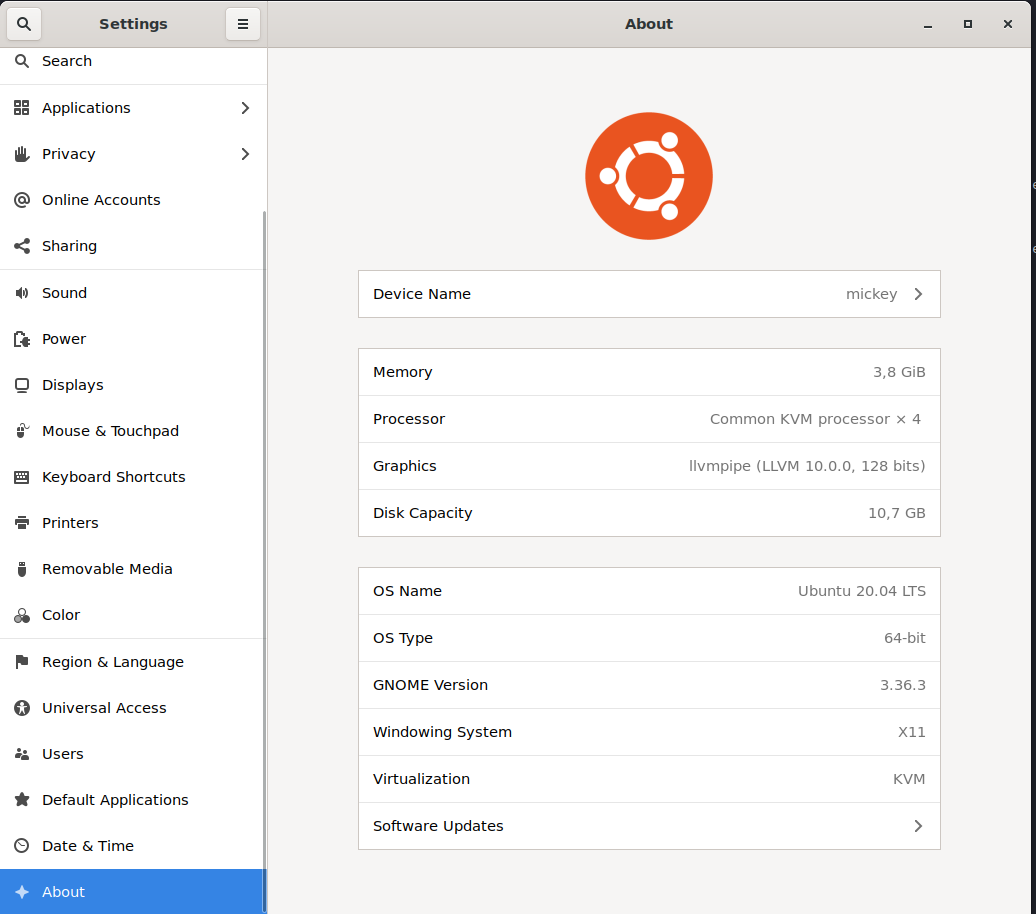
\includegraphics[width=0.85\textwidth]{./img/vuln13_mickey/gnome-control-center}
    \caption{Darstellung des \texttt{gnome-control-centers} von \texttt{Mickey}.}
    \label{gnome-control-center}
\end{figure}

\subsection{Risikobewertung}
Um den Angriff durchführen zu können, benötigt der Angreifer den Mitschnitt eines 4-Wege-Handshake des WPA-Protokolls. Da dieses jederzeit durch einen Angreifer duch eine Deauth-Attacke proviziert werden kann und der WPA2-Hashwert mit einer einfachen Wörterbuchattacke gebrochen werden kann, ist die Eintrittswahrscheinlichkeit für einen Angriff über die Luftschnittstelle mit HOCH zu bewerten. Darüber hinaus kann ein Angreifer sich mit dem angegriffenen WLAN verbinden. Sofern der Host \texttt{Mickey} ebenfalls im gleichen WLAN eingeloggt ist, so kann der Angreifer über SSH mit dem Benutzernamen \texttt{mickey} und dem WLAN-Passwort am Rechner \texttt{Mickey} anmelden. Da dieser Benutzer mittels \texttt{sudo} ebenfalls Root-Berechtigungen hat, ist die Schadenshöhe mit HOCH zu bewerten.

Das Gesamtrisiko wurde daher mit \textcolor{red}{HOCH} bewertet.

\subsection{Empfohlene Gegenmaßnahmen}
Das Passwort für das WLAN \texttt{Mickey's Office} sollte umgehend zu einem langen und komplexen Passwort geändert werden. Darüber hinaus wird empfohlen, die Authentifizierung auf WPA2-Enterprise (EAP) umzustellen. Das Passwort des Benutzers \texttt{mickey} auf dem Host \texttt{Mickey} sollte ebenfalls umgehend zu einem langen und komplexen Passwort geändert werden. Darüber hinaus sollten Passwörter nicht über Konten/Systeme hinweg benutzt werden, um die Angriffsfläche der Systeme im Falle einer Kompromittierung zu minimieren.

\subsection{Hinterlassene Spuren und Spurenbeseitigung}
Es wurden keine Dateien geändert, hinzugefügt oder Prozesse gestartet.
